\subsection{Endstufe}
\label{sec:endamp}
Der letzte Teil der Empfangseinheit besteht aus einem weiteren Verstärker und einem vorgeschalteten Hochpass. Der Hochpass hat eine Grenzfrequenz von $f_{g} \approx 1,59Hz$ und dient der Filterung vorangegangener DC-Offsets. Wie in Kapitel \ref{subsec:pre_amplifier} bereits gezeigt, ist die Verstärkung ausschließlich von den beiden Widerständen abhänging. Die Verstärkung der Endstufe ist somit über das Potentiometer von 0 bis 50 einstellbar.
\begin{figure}[H]
	\centering
	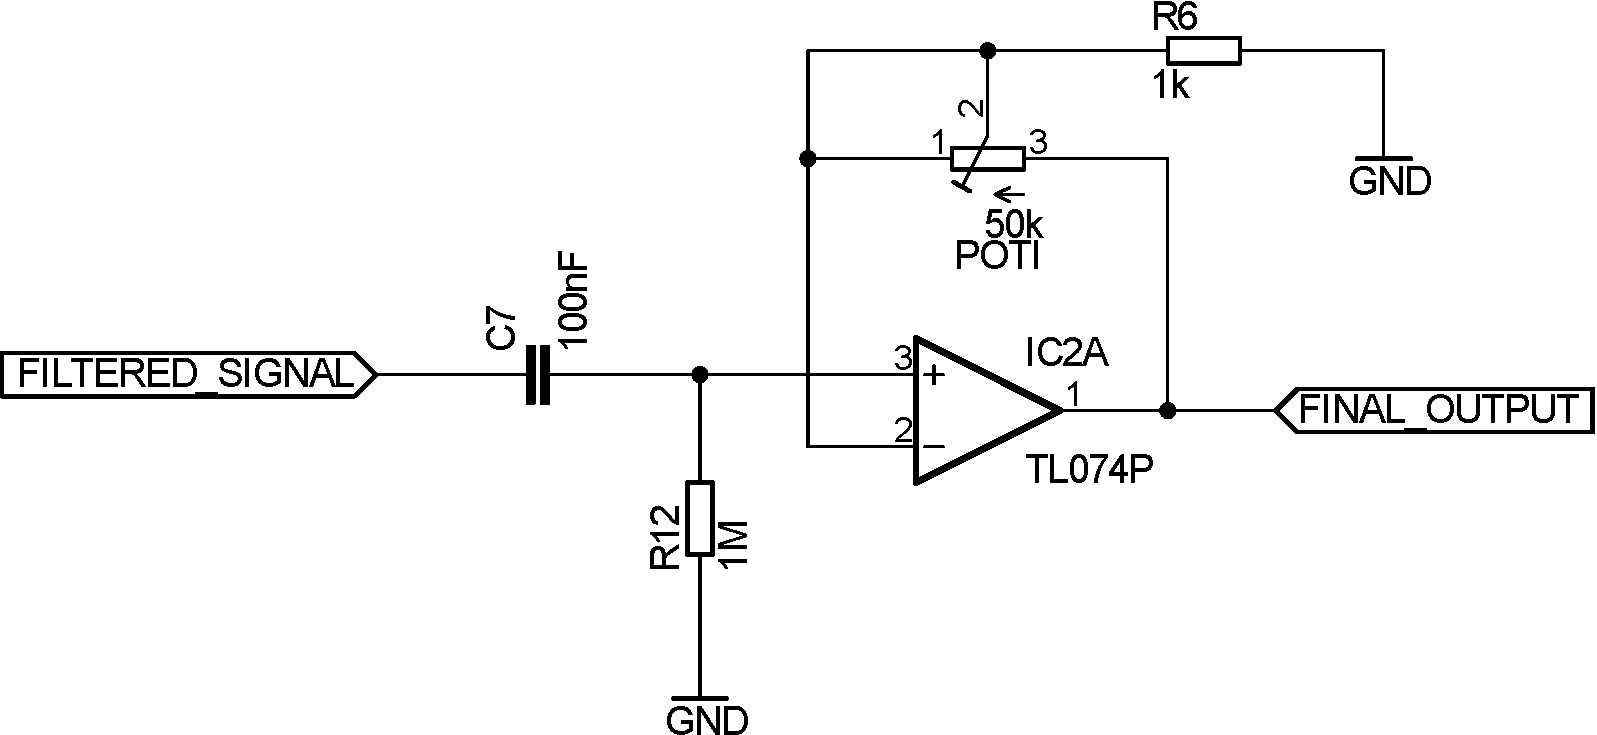
\includegraphics[scale=0.5]{gfx/post_amplifier.pdf}
	\caption{Endstufe}
	\label{fig:endamp}
\end{figure}